\chapter{Implementasi dan Pengujian}
\label{chap:implementasi dan pengujian}

Bab ini membahas tentang implementasi dan pengujian perangkat lunak berdasarkan rancangan yang sudah dibuat. Ada dua jenis pengujian yang dilakukan, yaitu pengujian fungsional dan pengujian eksperimental. Bab ini juga membahas tentang lingkungan yang digunakan untuk pengujian perangkat lunak ini.

\section{Lingkungan untuk Pengujian}
Pengujian fungsional dan pengujian eksperimental dilakukan menggunakan dua jenis lingkungan yang berbeda. 
\begin{enumerate}
	\item Pengujian Fungsional. \\
	Berikut spesifikasi perangkat keras dan perangkat lunak yang digunakan untuk melakukan pengujian fungsional
	\begin{table}[H] %atau h saja untuk "kira kira di sini" 
		\caption{Lingkungan perangkat keras untuk pengujian fungsional}
		\label{tab:lingkunganpkpf}
		\resizebox{\textwidth}{!}{%
			\begin{tabular}{|l|l|}
				\hline
				\textbf{Parameter} & \textbf{Nilai} \\
				\hline
				\textit{Processor} & \textit{Intel Core i5 4200u}\\
				\hline
				\textit{Graphics Processing Unit (GPU)} & \textit{Intel HD Graphics HD4000} dan \textit{Nvidia GeForce 840M}\\
				\hline
				\textit{Random Access Memory (RAM)}& 12.00GB DDR3\\
				\hline
				\textit{Storage} & 120GB \textit{SSD} dan 1TB \textit{Harddisk}\\
				\hline
		\end{tabular}}
	\end{table}

	\begin{table}[H] %atau h saja untuk "kira kira di sini" 
		\caption{Lingkungan perangkat lunak untuk pengujian fungsional}
		\label{tab:lingkunganplpf}
		\resizebox{\textwidth}{!}{%
			\begin{tabular}{|l|l|}
				\hline
				\textbf{Parameter} & \textbf{Nilai} \\
				\hline
				Sistem Operasi & Windows 10 \textit{10 Education 64-bit}\\
				\hline
				Bahasa Pemrograman & PHP, JavaScript, CSS dan HTML\\
				\hline
				\textit{Text Editor} & \textit{Atom}\\
				\hline
				\textit{Framework} & \textit{CodeIgniter}\\
				\hline
				\multirow{4}{*}{Perangkat Lunak pendukung} 	& \textit{XAMPP Control Panel} v3.2.2\\
															& \textit{Google Chrome Version} 65.0.3325.181 (Official Build) (64-bit)\\
															& \textit{Firefox Quantum} 59.0.2 (64-bit)\\
															& \textit{Microsoft Excel} 2016\\
				\hline
		\end{tabular}}
	\end{table}

	\item Pengujian Eksperimental. \\
	Berikut spesifikasi perangkat keras dan perangkat lunak yang digunakan untuk melakukan pengujian eksperimental
	\begin{table}[H] %atau h saja untuk "kira kira di sini" 
		\caption{Lingkungan perangkat keras untuk pengujian eksperimental}
		\centering
		\label{tab:lingkunganpkpe}
		%\resizebox{\textwidth}{!}
	\end{table}
	
	\begin{table}[h] %atau h saja untuk "kira kira di sini" 
		\caption{Lingkungan perangkat lunak untuk pengujian eksperimental}
		\label{tab:lingkunganplpe}
		\centering
		%\resizebox{\textwidth}{!}
	\end{table}
\end{enumerate}

\section{Implementasi}
Hasil implementasi dari rancangan perangkat lunak yang sudah dibuat ini terdiri dari tiga bagian, yaitu
\begin{enumerate}
	\item Kode program \\
	Perubahan dan penambahan kode program untuk mengimplementasi kebutuhan \textit{Sharif Judge}, ditulis dalam bahasa pemrograman PHP. Seluruh perubahan kode program telah dijabarkan dalam setiap sub bab pada bab 4. Kode program untuk halaman \textit{Logs} dan \textit{Hall of Fame} dapat dilihat di bab Lampiran --.
	\item Basis Data \\
	Terdapat penambahan \textit{key} dan \textit{value} dalam mengimplementasi kebutuhan \textit{Sharif Judge} pada sub bab 4.7. Pada tabel \textit{shj\_settings} ditambahkan \textit{shj\_key} dengan nama \textit{lock\_student\_display\_name} dan \textit{shj\_value} dengan nilai 0. Berikut struktur tabel \textit{shj\_settings}
	
	\begin{table}[H] %atau h saja untuk "kira kira di sini"
		\centering 
		\caption{Struktur Tabel \textit{shj\_settings}}
		\label{tab:atributtabelsettings}
		\resizebox{\textwidth}{!}{
		\begin{tabular}{|c|c|}
			\hline
			\textbf{shj\_key} & \textbf{shj\_value}\\
			\hline
			\textit{timezone} & Asia/Jakarta\\
			\hline
			\textit{tester\_path} & path{C:/xampp/htdocs/tester}\\
			\hline
			\textit{assignments\_root} & path{C:/xampp/htdocs/assignments}\\
			\hline
			\textit{file\_size\_limit} & 50\\
			\hline
			\textit{output\_size\_limit} & 1024\\
			\hline
			\textit{queue\_is\_working} & 0\\
			\hline
			\textit{default\_late\_rule} & /** Put coefficient (from 100) in variable \$co...\\
			\hline
			\textit{enable\_easysandbox} & 1\\
			\hline
			\textit{enable\_c\_shield} & 1\\
			\hline
			\textit{enable\_cpp\_shield} & 1\\
			\hline
			\textit{enable\_py2\_shield} & 1\\
			\hline
			\textit{enable\_py3\_shield} & 1\\
			\hline
			\textit{enable\_java\_policy} & 1\\
			\hline
			\textit{enable\_log} & 1\\
			\hline
			\textit{submit\_penalty} & 300\\
			\hline
			\textit{enable\_registration} & 1\\
			\hline
			\textit{registration\_code} & 0\\
			\hline
			\textit{mail\_from} & shj@example.com\\
			\hline
			\textit{mail\_from\_name} & \textit{Sharif Judge}\\
			\hline
			\textit{reset\_password\_mail} & <p> Someone requested a password reset for your S...\\
			\hline
			\textit{add\_user\_mail} & <p> Hello! You are registered in SharIF Judge at ...\\
			\hline
			\textit{moss\_userid} & \\
			\hline
			\textit{results\_per\_page\_all} & 40\\
			\hline
			\textit{results\_per\_page\_final} & 80\\
			\hline
			\textit{week\_start} & 0\\
			\hline
			\textit{lock\_student\_display\_name} & 1\\
			\hline
		\end{tabular}}
	\end{table}
	
	Terdapat penambahan atribut dalam mengimplementasi kebutuhan \textit{Sharif Judge} pada sub bab 4.8. Pada tabel \textit{shj\_assignments} ditambahkan atribut baru dengan nama \textit{archived\_assignment}. Berikut struktur tabel \textit{shj\_assignments}
	
	\begin{table}[H] %atau h saja untuk "kira kira di sini"
		\centering 
		\caption{Struktur Tabel \textit{shj\_assignments}}
		\label{tab:atributtabelassignments}
		%\resizebox{\textwidth}{!}{
		\begin{tabular}{|c|c|c|c|}
			\hline
			\textbf{Atribut} & \textbf{Tipe Data} & \textbf{Ukuran}  & \textbf{Default} \\
			\hline
			\textit{id (primary key)} & int & 11  & None \\
			\hline
			\textit{name} & varchar & 50  & - \\
			\hline
			\textit{problems} & smallint & 4  & None \\
			\hline
			\textit{total\_submits} & int & 11  & None \\
			\hline
			\textit{open} & tinyint & 1  & None \\
			\hline
			\textit{scoreboard} & tinyint & 1  & None \\
			\hline
			\textit{javaexceptions} & tinyint & 1  & None \\
			\hline
			\textit{description} & text & -  & None \\
			\hline
			\textit{start\_time} & datetime & 1  & None \\
			\hline
			\textit{finish\_time} & datetime & 1  & None \\
			\hline
			\textit{extra\_time} & int & 11  & None \\
			\hline
			\textit{late\_rule} & text & -  & None \\
			\hline
			\textit{participants} & text & -  & None \\
			\hline
			\textit{moss\_update} & varchar & 30  & None \\
			\hline
			\textit{archived\_assignment} & tinyint & 1  & None \\
			\hline
		\end{tabular}%}
	\end{table}

	Terdapat penambahan tabel dalam mengimplementasi kebutuhan \textit{Sharif Judge} pada sub bab 4.5. Tabel tersebut diberi nama \textit{shj\_logins}. Berikut struktur tabel \textit{shj\_logins}
	\begin{table}[H] %atau h saja untuk "kira kira di sini"
		\centering 
		\caption{Struktur Tabel \textit{shj\_logins}}
		\label{tab:tabellogsfix}
		\begin{tabular}{|c|c|c|c|}
			\hline
			\textbf{Atribut} & \textbf{Tipe Data} & \textbf{Ukuran}  & \textbf{Default} \\
			\hline
			\textit{login\_id (primary key)} & int & 11  & None \\
			\hline
			\textit{username} & varchar & 20  & None \\
			\hline
			\textit{ip\_address} & varchar & 15  & None \\
			\hline
			\textit{timestamp} & timestamp & 11  & current\_timestamp \\
			\hline
			\textit{last\_24h\_login\_id}	 & int & 11  & null \\
			\hline
		\end{tabular}
	\end{table}

	\item Tampilan \\
	Tampilan untuk untuk pengembangan Sharif Judge ini dirancang bedasarkan rancangan tampilan yang sudah dibuat. Berikut beberapa tampilan halaman baru pada pengembangan Sharif Judge
	
	\begin{figure}[H]
		\centering  
		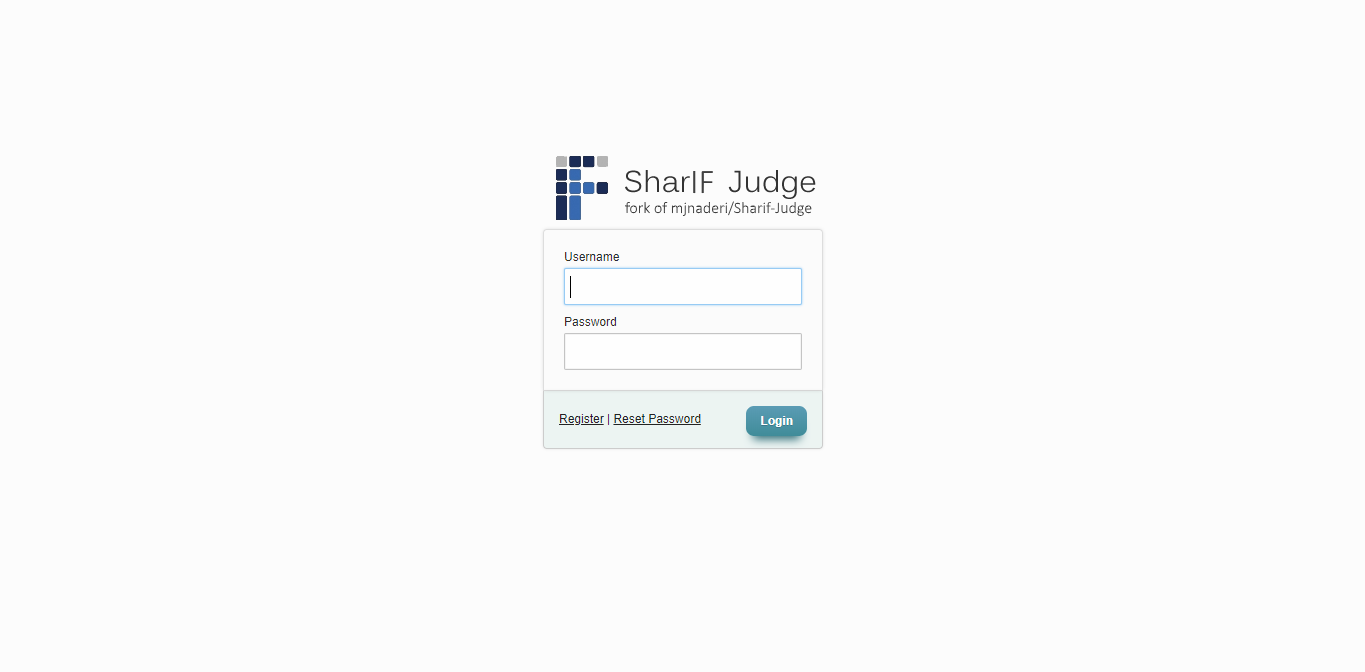
\includegraphics[width=1.0\textwidth]{newlogin}  
		\caption[Tampilan Halaman Login]{Tampilan Halaman Login} 
		\label{fig:newlogin} 
	\end{figure}
	
	\begin{figure}[H]
		\centering  
		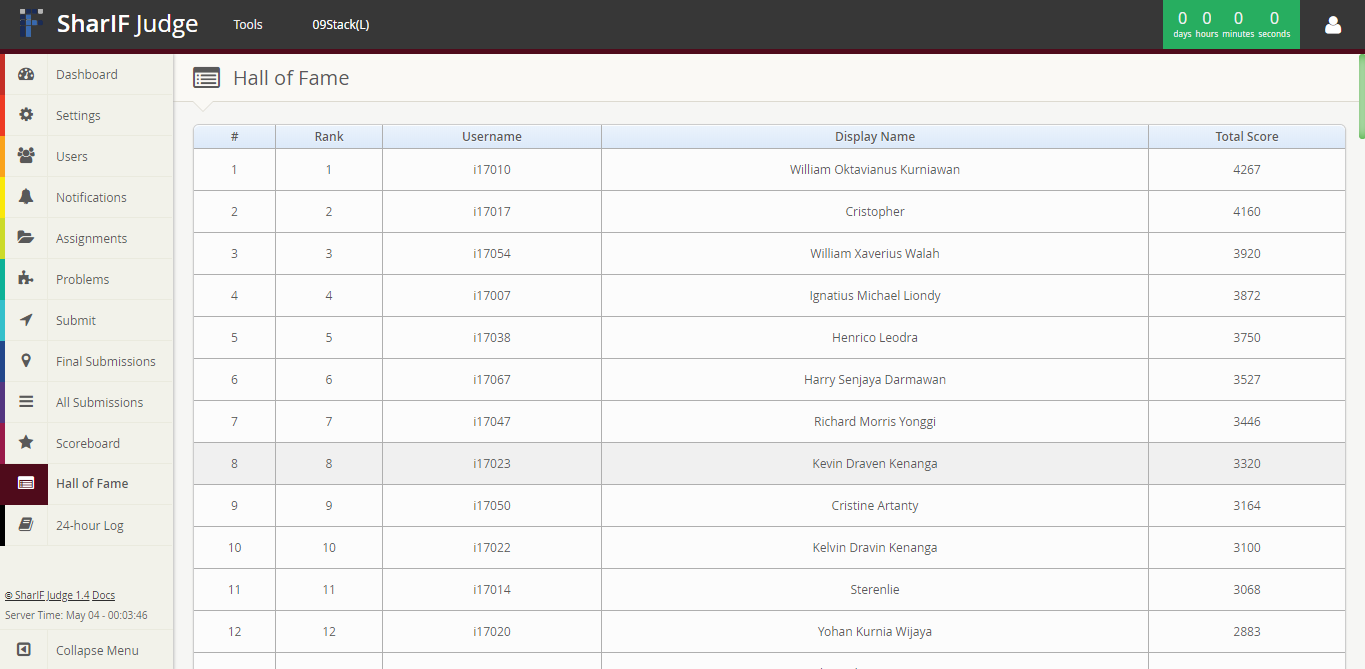
\includegraphics[width=1.0\textwidth]{newhof}  
		\caption[Tampilan Halaman Hall of Fame]{Tampilan Halaman Hall of Fame} 
		\label{fig:newhof} 
	\end{figure}

	\begin{figure}[H]
		\centering  
		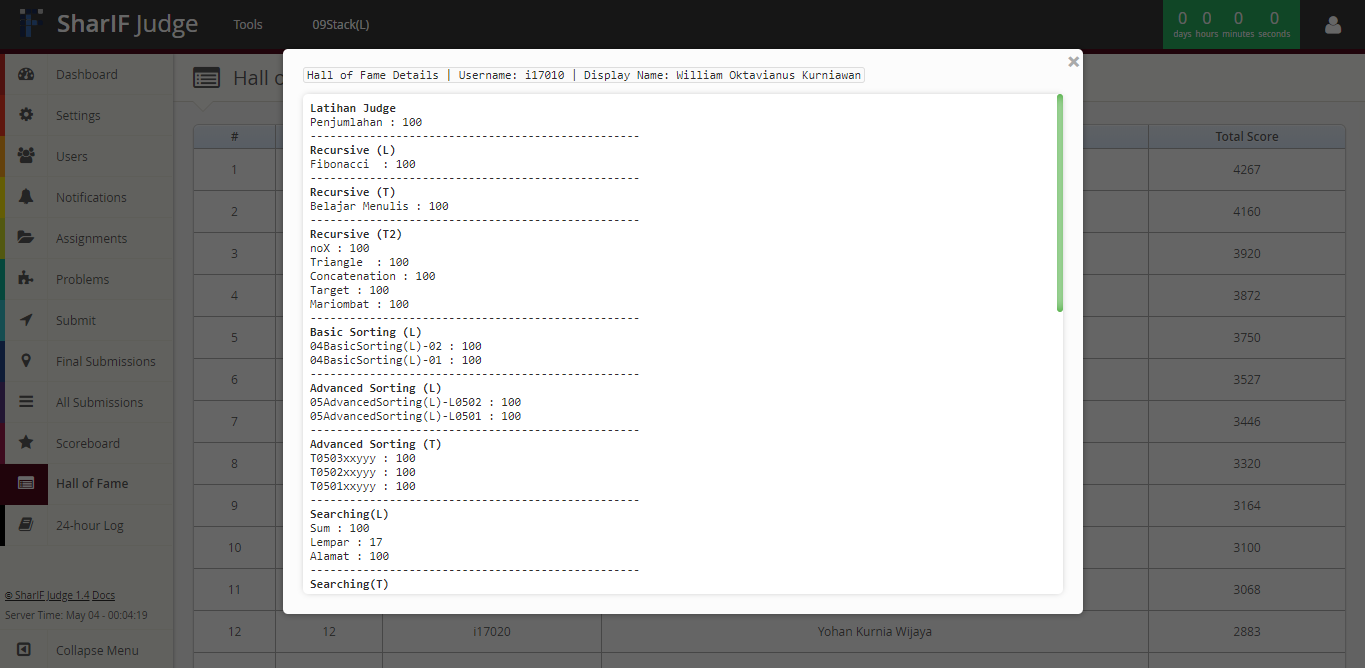
\includegraphics[width=1.0\textwidth]{newhofdetail}  
		\caption[Tampilan Detail dari Hall of Fame]{Tampilan Detail dari Hall of Fame} 
		\label{fig:newhofdetail} 
	\end{figure}

	\begin{figure}[H]
		\centering  
		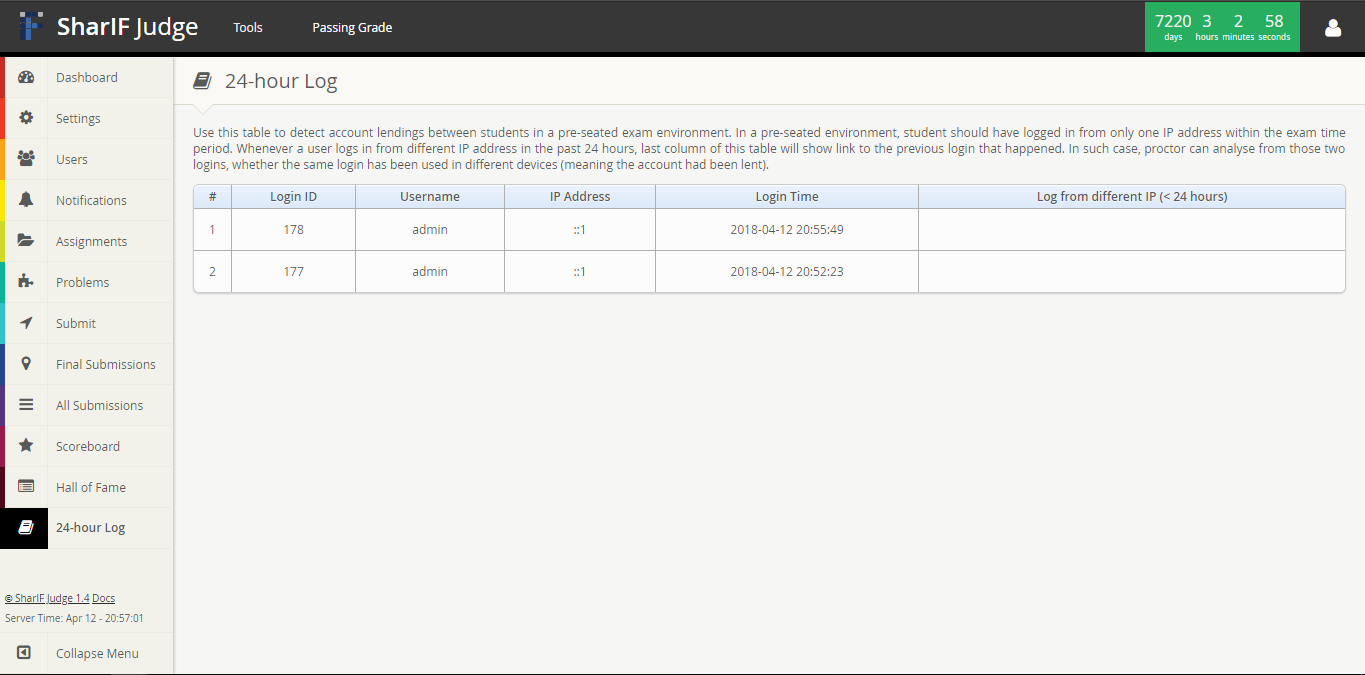
\includegraphics[width=1.0\textwidth]{newlogs}  
		\caption[Tampilan Halaman Logs]{Tampilan Halaman Logs} 
		\label{fig:newlogs} 
	\end{figure}

	\begin{figure}[H]
		\centering  
		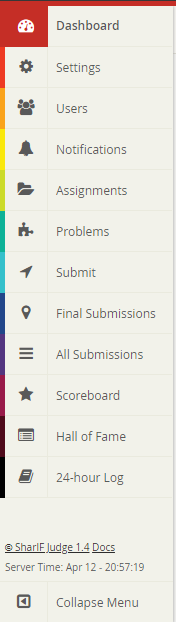
\includegraphics[scale=0.7]{sidemenu}  
		\caption[Tampilan Side Menu]{Tampilan Side Menu} 
		\label{fig:sidemenu} 
	\end{figure}
\end{enumerate}